\section{Performance of the Spherical Harmonics Analysis in Separating 0\nbb-decay from \B~Background.}
\label{sec:performance}

In this section we discuss factors that affect performance of the spherical harmonics technique in separating
0\nbb~signal from \B~background events. We found that most separation comes from the first two multiple moments,
$l=0$ and $l=1$. However, according to Eq.~\ref{eq6}, higher multiple moments are needed for a better normalization of the 
power spectrum $S_l$. In the following we choose to calculate power spectrum $s_l$ up to multiple moment of l=3 and
use only normalized variable $S_0$ and $S_1$, where the normalization is given by

\begin{eqnarray}
\label{eq7}
S_{0,1} = \frac{s_{0,1}}{\sum_{l=0}^{3} s_l}
\end{eqnarray}

As discussed below, a linear combination of $S_0$ and $S_1$ can be used to construct a single variable, $S_{01}$, that provides 
separation between signal and background in 1D space. We show distributions of this variable $S_{01}$ to demonstrate qualitatively 
the separation between 0\nbb~and \B~events depending on a few key assumptions about the detector characteristics.

Since the goal of this paper is to describe the technique of spherical harmonics analysis for separating
different event topologies relevant for 0\nbb-decay searches in a generic liquid scintillator detector, we intentionally refrain from any 
quantitative estimates on the improvements in sensitivity to 0\nbb~decay. The actual improvements in sensitivity due to spherical 
harmonics analysis would depend on various details of a given experimental setup. Therefore, we believe that detailed qunatitative 
sensitivity studies are more apporpiate in the context of a particular 0\nbb~decay experiment which is beyond the scope of this paper.

\subsection{Central events with perfect vertex reconstruction}

We start evaluating the performance of the sphercical harmonics analysis from looking into events that originate at the center
of the detector and assuming perfect reconstruction of the event vertex position. For such events, a time cut of 33.5~ns on PEs 
arrival time can be applied to obtain early PEs sample which contain high fraction of Cherenkov PE. The default QE and 100\% 
photo-coverage is used in the simulation.

Comparison of $S_0$ and $S_1$ distributions for 0\nbb-decay signal and \B~background events is shown in Fig.~\ref{fig:S_vs_energy}.
Both variables provide a noticeable separation between signal and background. We also note that in the energy range of interest, 
the $S_l$'s do not strongly depend on the energy deposited in the detector, which makes information contained in the normalized power 
spectrum complimentary to the energy measurements. Therefore, spherical harmonics analysis can be used as an additional handle for
background suppresion at the end point of the 0\nbb-decay energy spectrum.

\begin{figure*}[h]
\centering
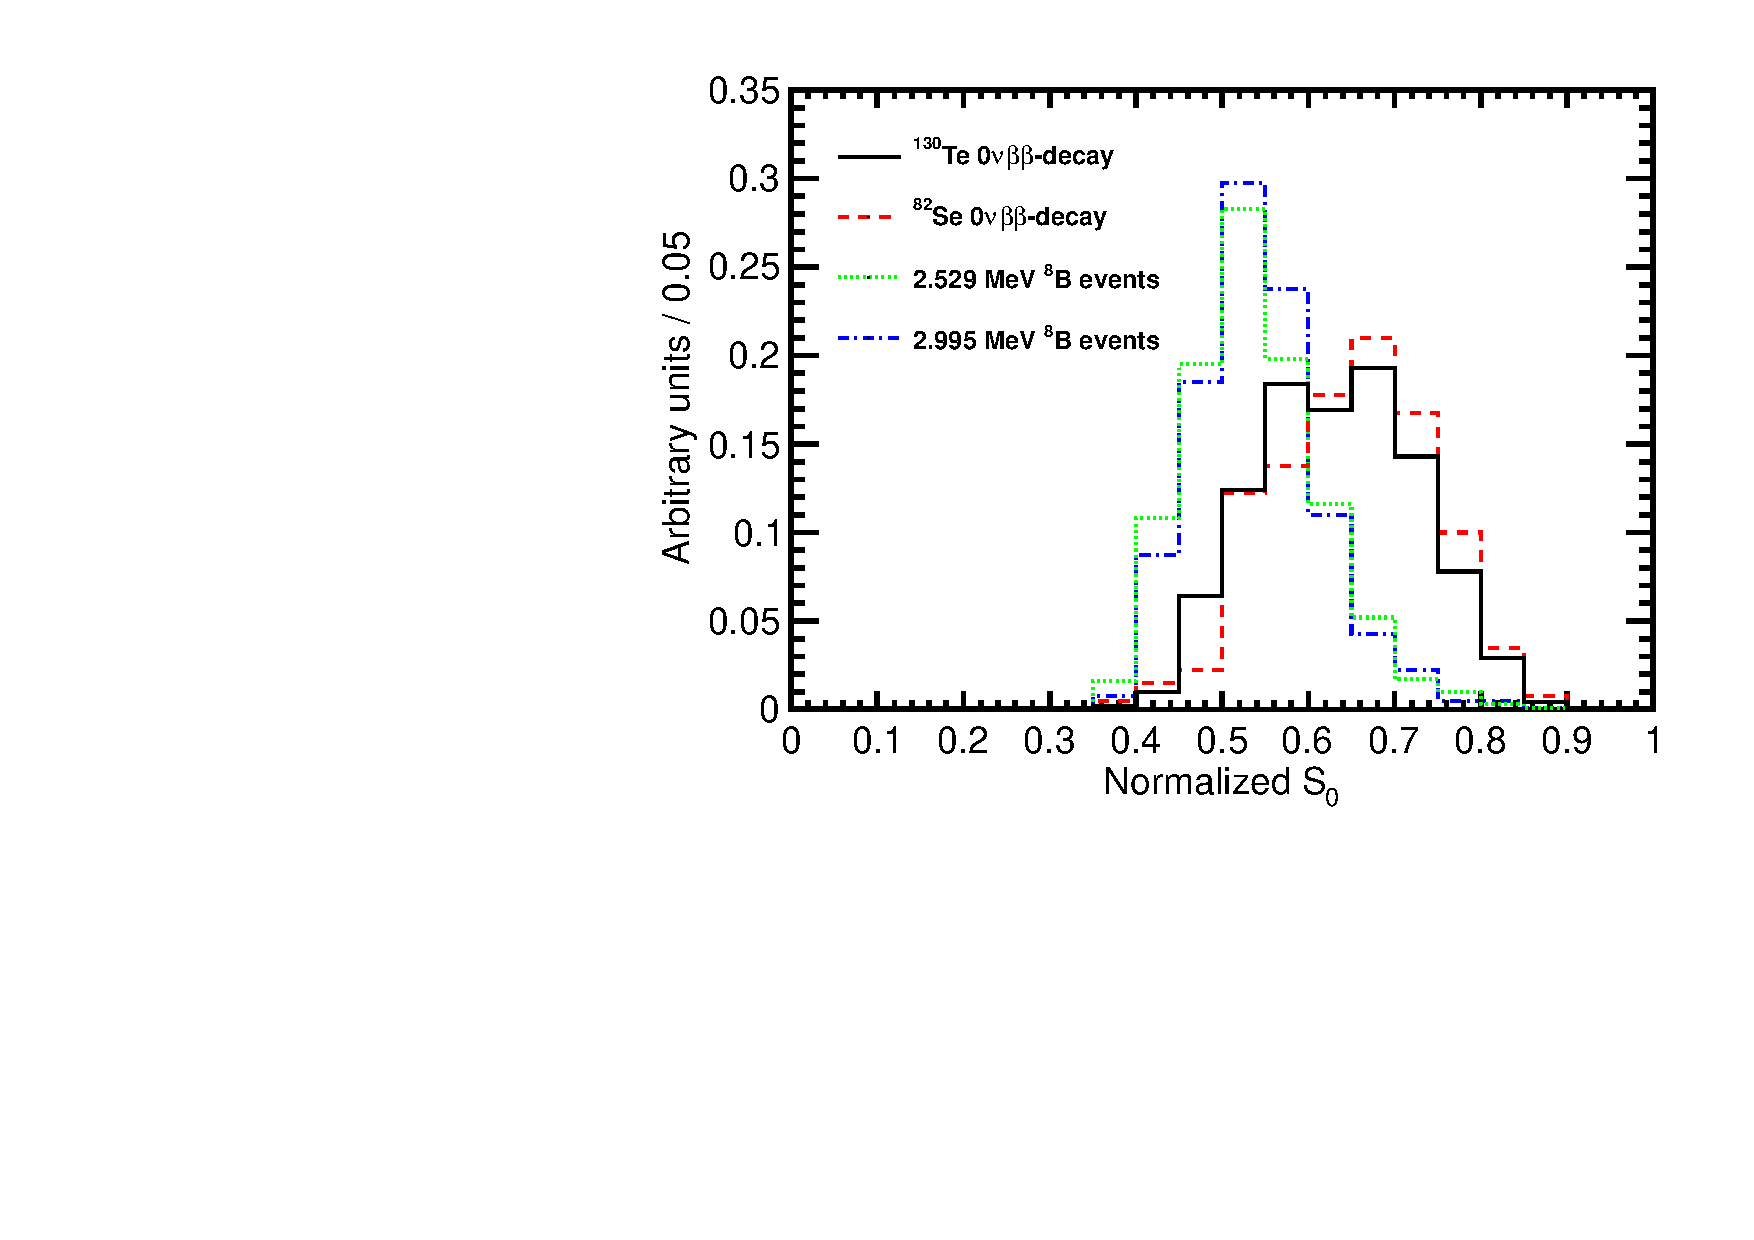
\includegraphics[width=0.49\textwidth]{hS0.pdf}
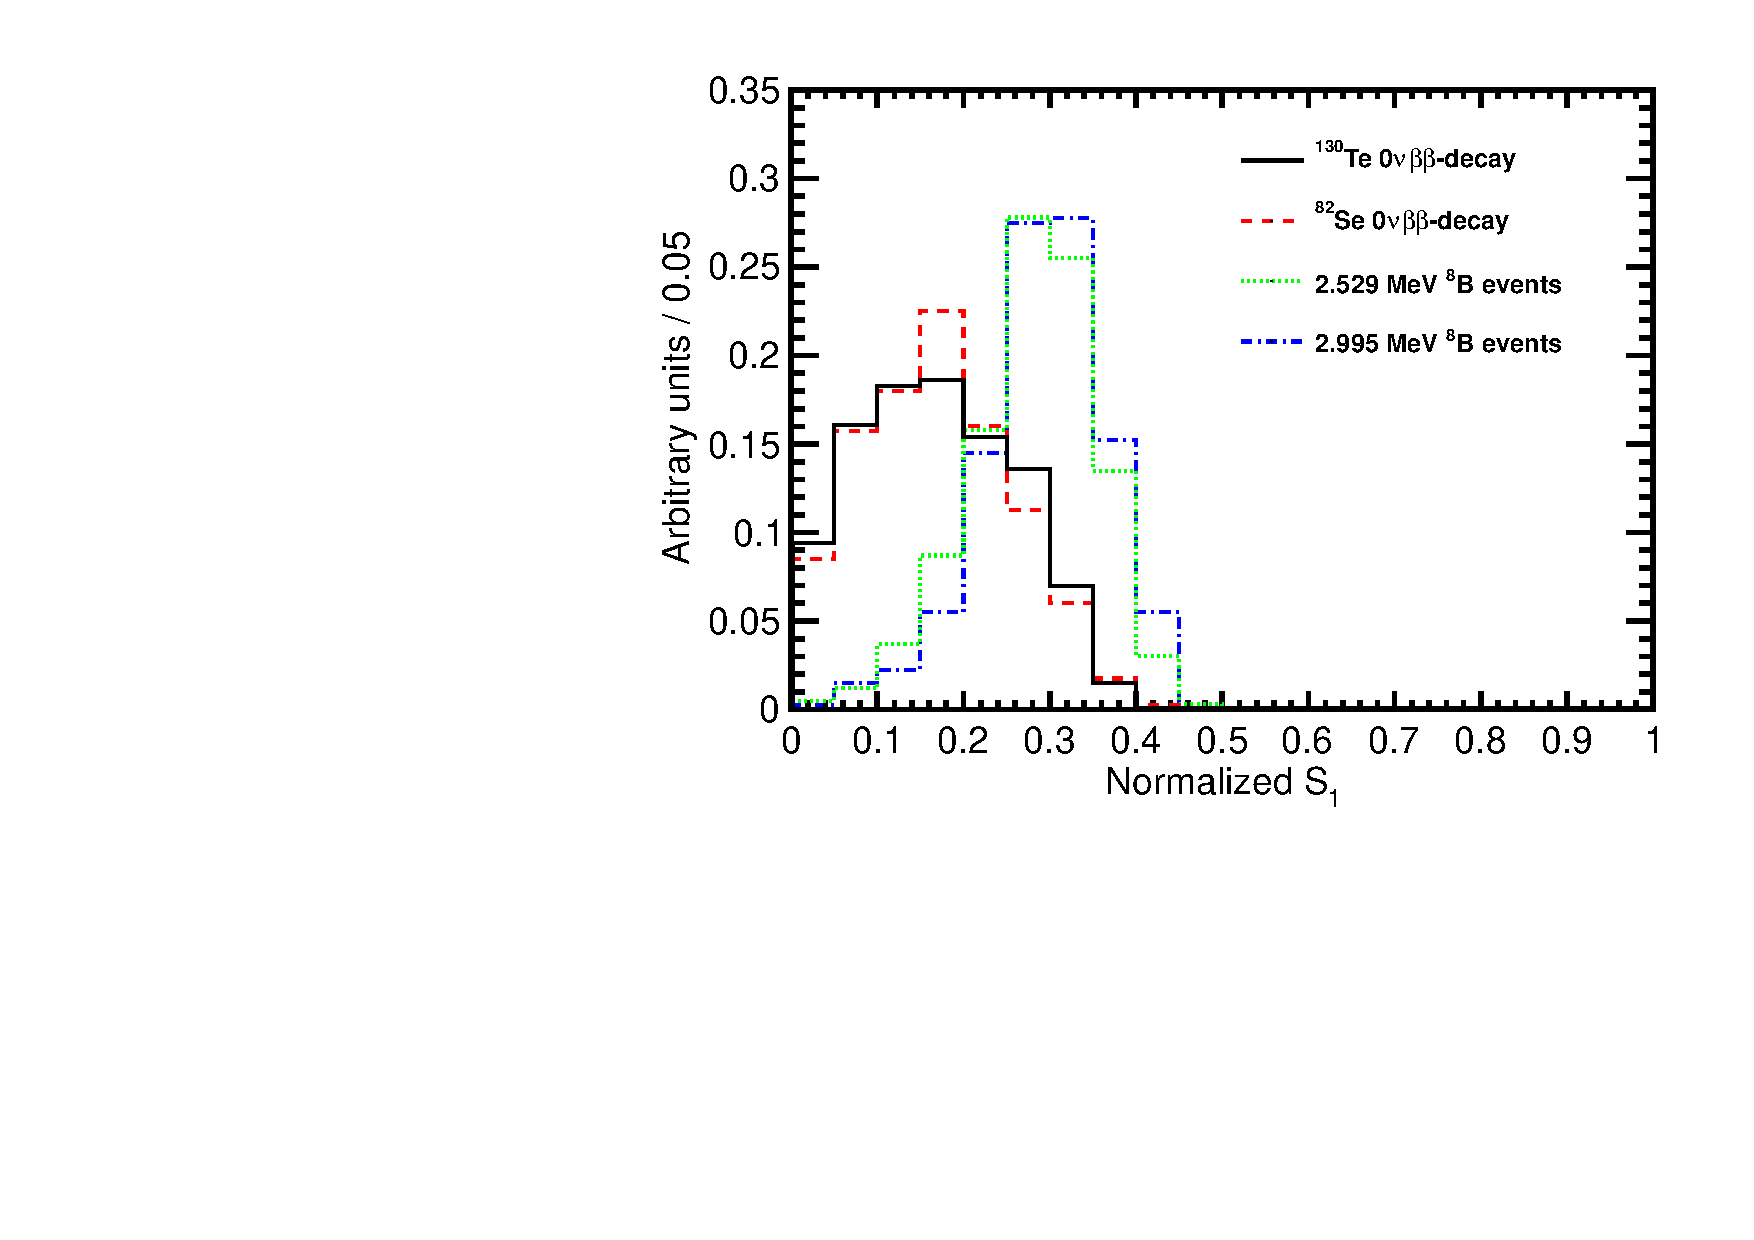
\includegraphics[width=0.49\textwidth]{hS1.pdf}
\caption{$S_0$ (\emph{left}) and $S_1$ (\emph{right}) distributions for 1000 simulated 0\nbb-decay signal and \B~background events.
  Two different isotopes are compared, $^{130}$Te and $^{82}$Se. Corresponding kinetic energies of \B~single electrons are
  2.53 MeV and 3.00 MeV. Central events assuming perfect reconstruction of vertex position. Time cut of 33.5~ns on the PE arrival time is
  applied. The default QE and 100\% photo-coverage is used in the simulation.}
\label{fig:S_vs_energy}
\end{figure*}

Left panel in Fig.~\ref{fig:SL_Te_33p5ns_center} compares scatter plots of the first two components of the power spectrum, 
$S_0$ and $S_1$, for signal and background. In order to optimize separation between $^{130}$Te and $^{8}$B
events, a linear combination of $S_0$ and $S_1$, $S_{01}$, is constructed as follows. 

First, a linear fit, $S_0$ = $A \cdot S_1 + B$, of all points on the scatter plot is performed as shown by the dashed 
line in the left panel of Fig.~\ref{fig:SL_Te_33p5ns_center}. Then a 1-D variable $S_{01}$ is defined as
$S_{01} = S_1 \cdot cos(\theta) + S_0 \cdot sin(\theta)$, where $tan(\theta)$=$A$. Right panel in Fig.~\ref{fig:SL_Te_33p5ns_center}
compares distributions of $S_{01}$ for 0\nbb-decay signal and \B~background. These 1-D histogrmas for $S_{01}$ represent
projection of points on the scater plot onto the fitted line. We use distribution of the variable $S_{01}$ as a figure of merit
for signal/background separation. We conclude that spherical harmonics analysis potentialy brings new separation power that is
in addition to energy measusrements.


\begin{figure*}[h]
  \centering
  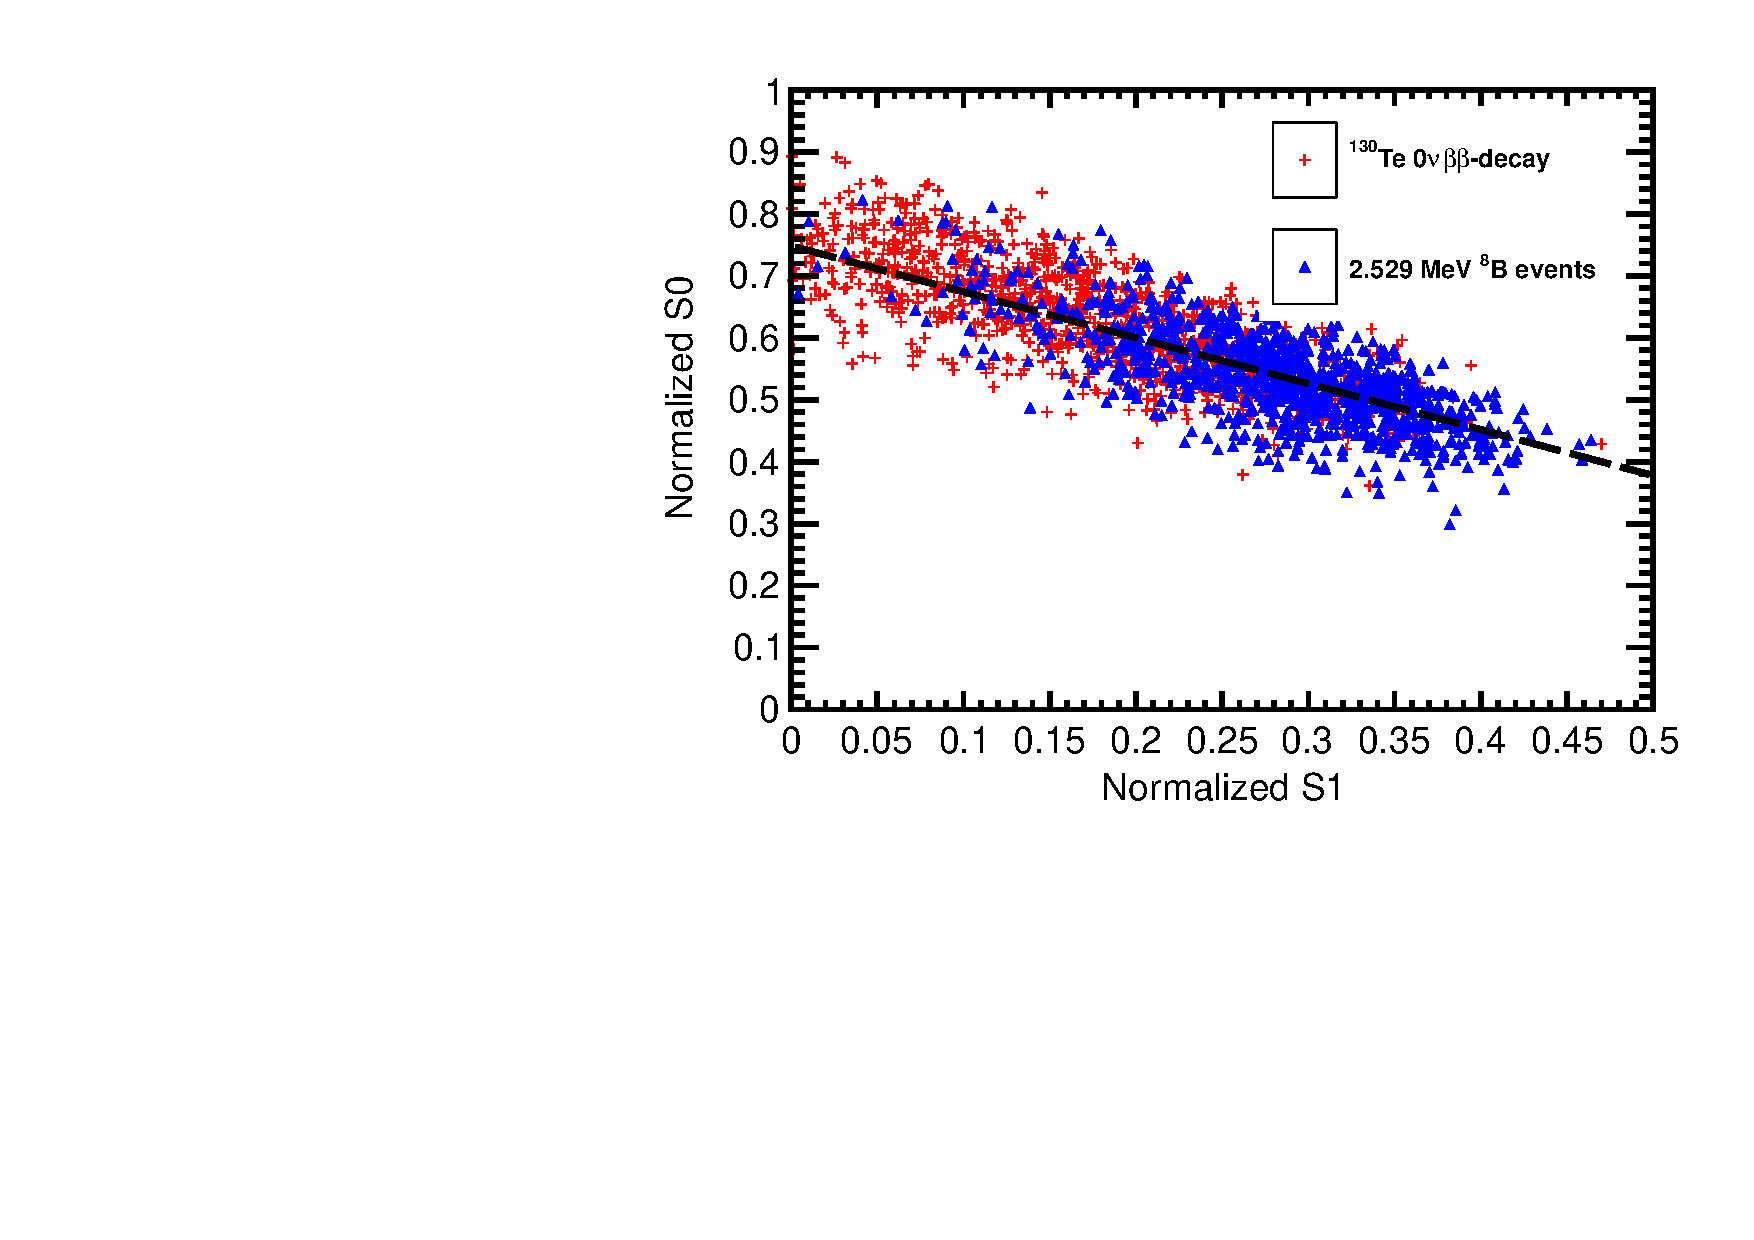
\includegraphics[width=0.49\textwidth]{hS0vsS1_Te130_1el_allLight_VtxSmear0cm_VtxShiftX0cm_33p5ns_center.pdf}
%  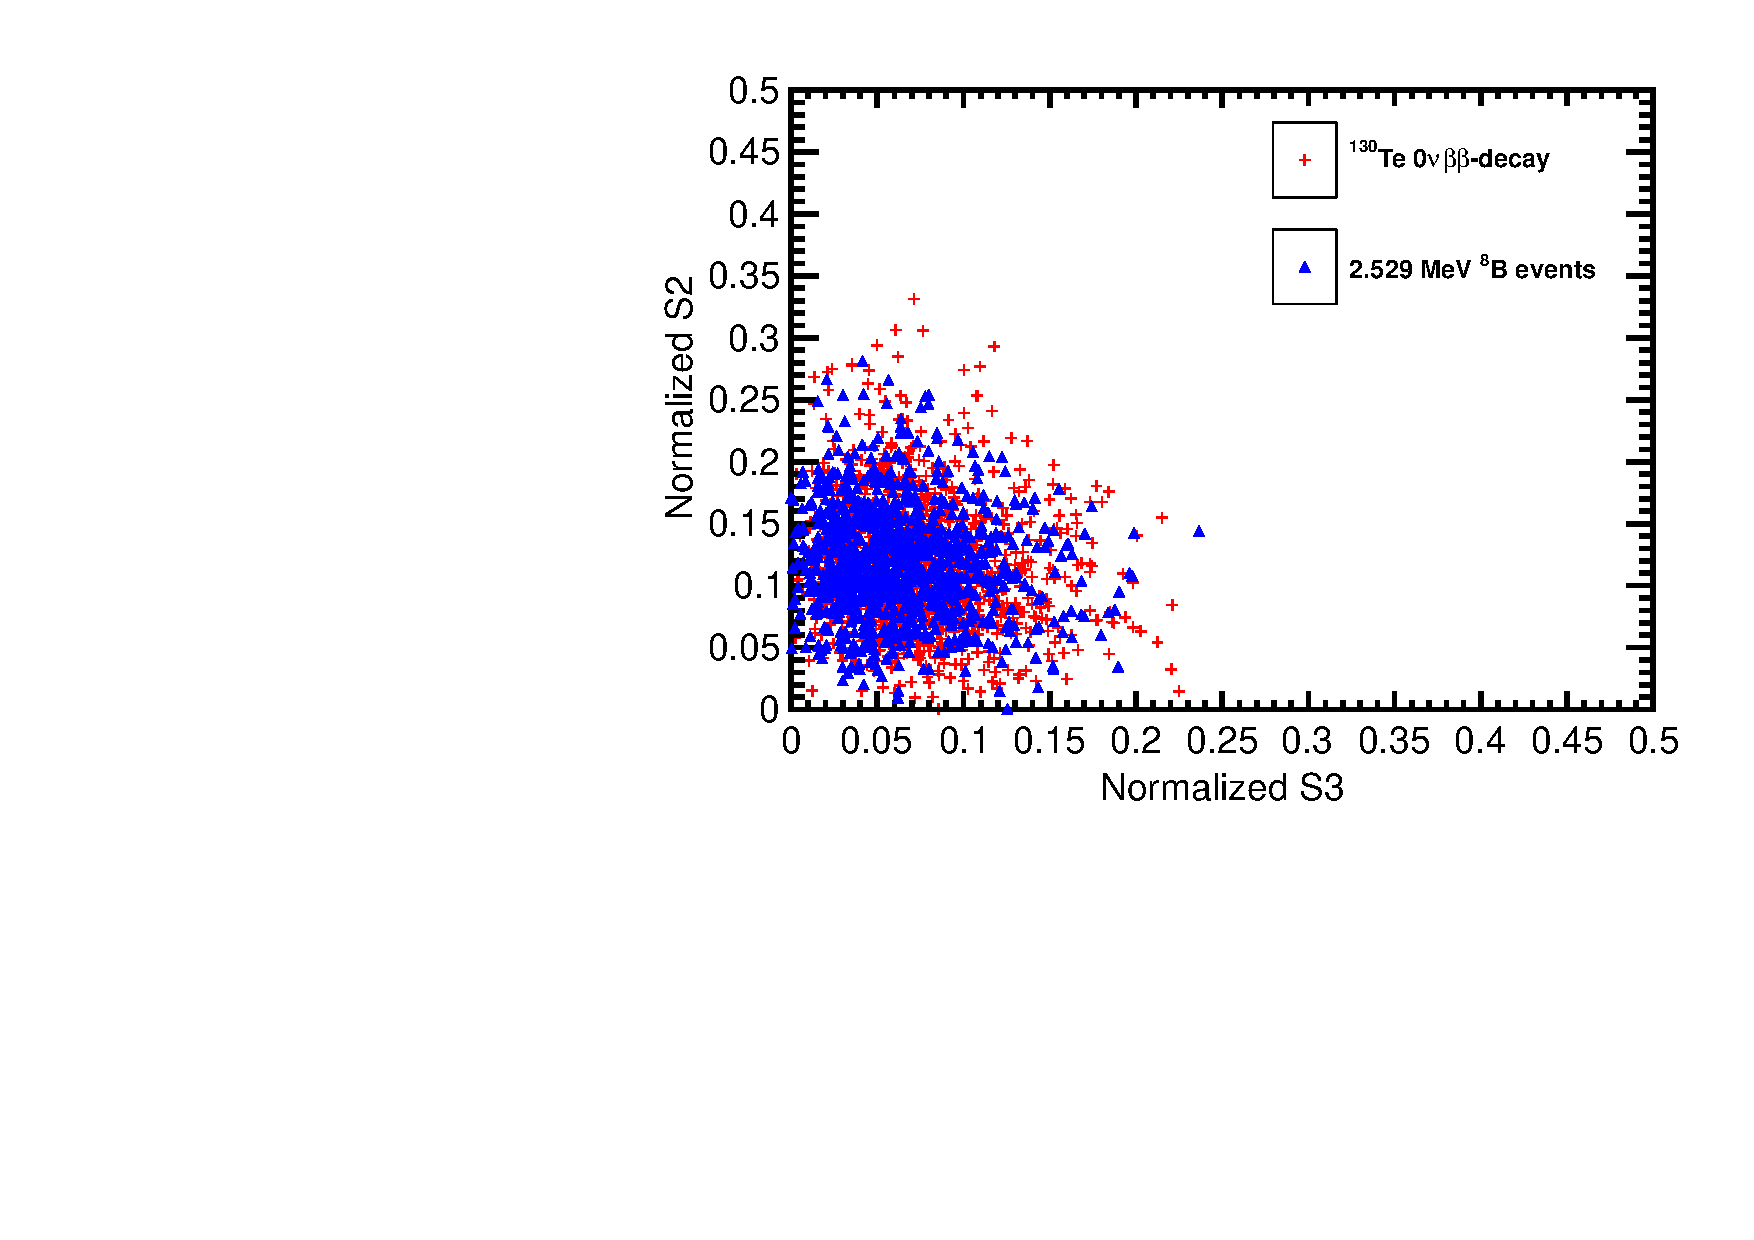
\includegraphics[width=0.49\textwidth]{hS2vsS3_Te130_1el_allLight_VtxSmear0cm_VtxShiftX0cm_33p5ns_center.pdf}
  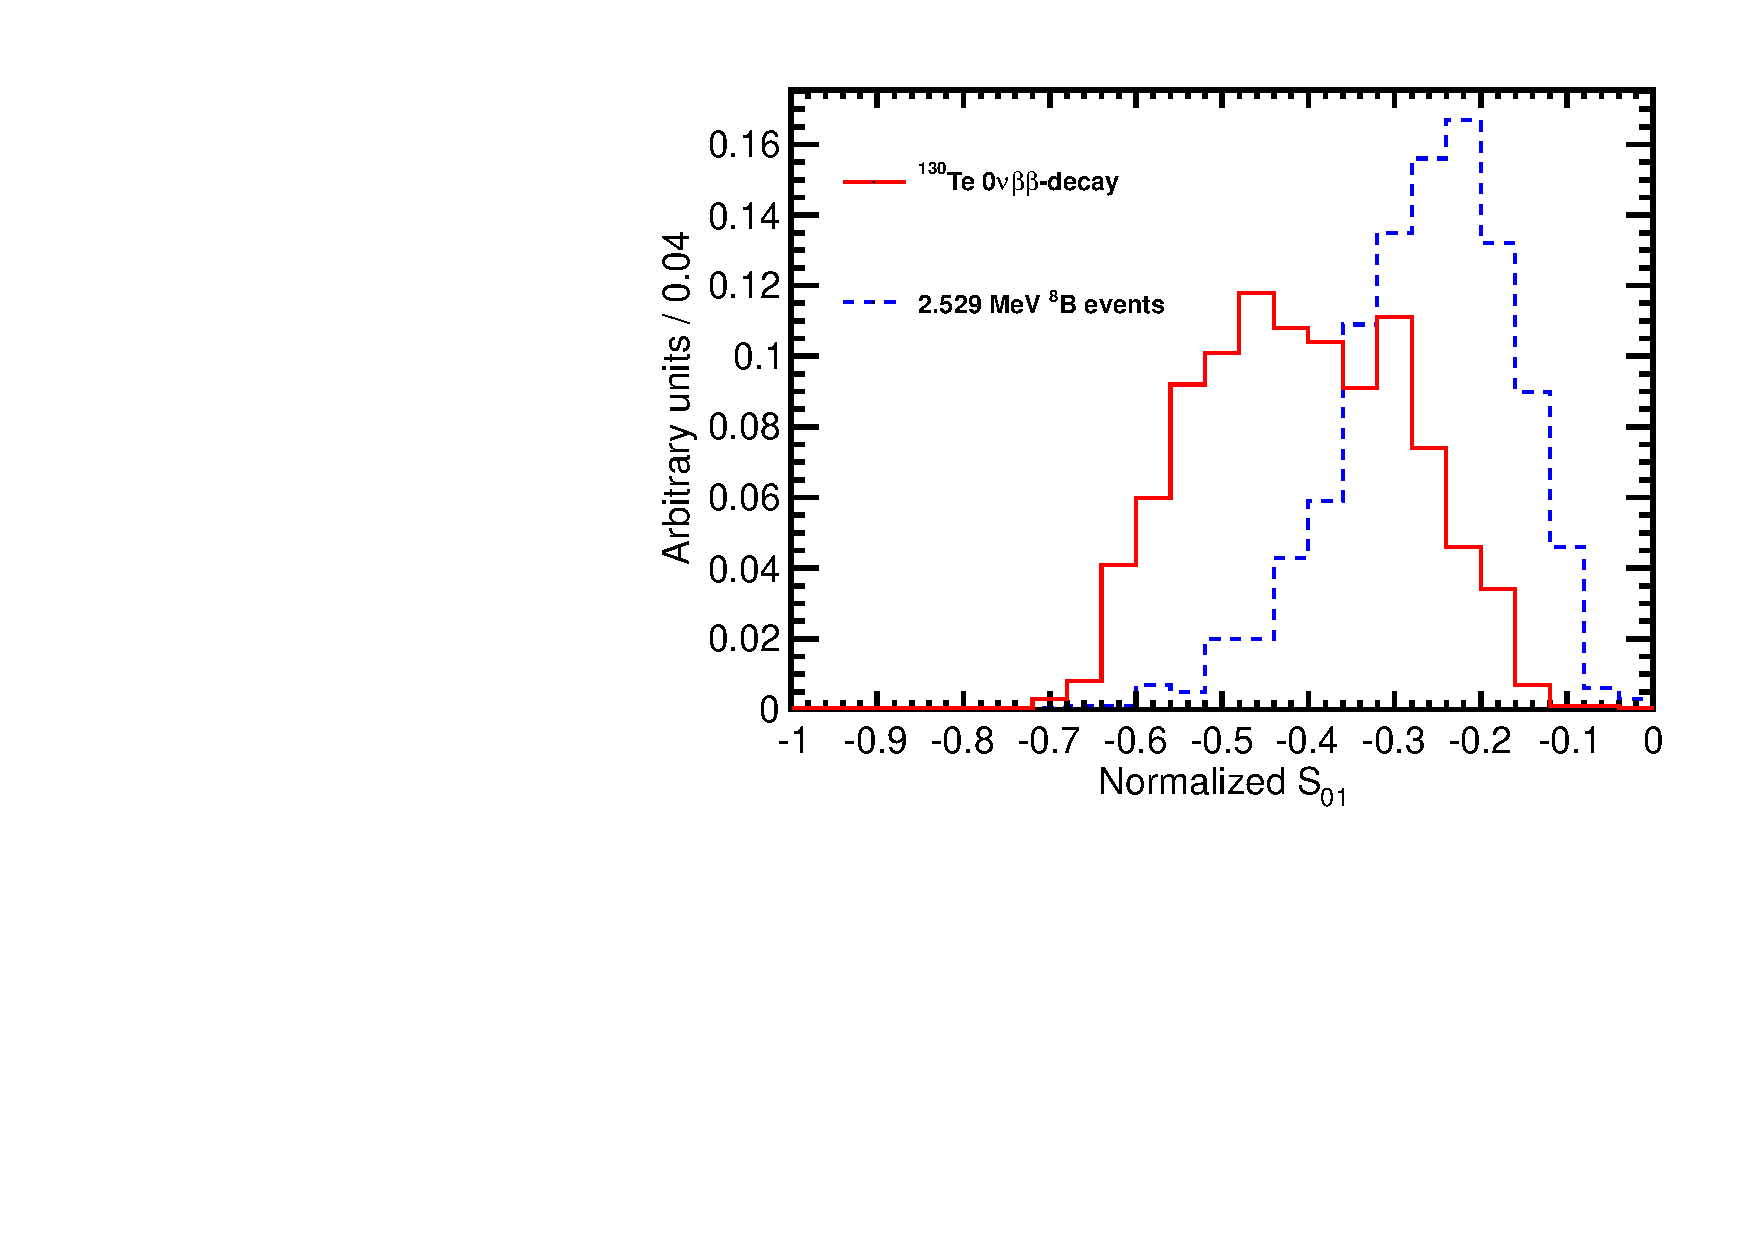
\includegraphics[width=0.49\textwidth]{hS01_allLight_VtxSmear0cm_VtxShiftX0cm_33p5ns_center.pdf}
  \caption{\emph{Left:} Scatter plot of $S_0$ versus $S_1$ for a simulation of 1000 signal (\emph{red crosses}) and background 
    (\emph{blue triangles}) events.
    Central events assuming perfect reconstruction of vertex position. Time cut of 33.5~ns on the PE arrival time is
    applied. The default QE and 100\% photo-coverage is used in the simulation.
    Black dashed line corresponds to a linear fit to define 1-D variable $S_{01}$ (see text for details).
    \emph{Right:} Comparison of the $S_{01}$ distribution between signal (\emph{red solid line}) and background (\emph{blue dashed line}).}
\label{fig:SL_Te_33p5ns_center}
\end{figure*}



\subsection{Experimental challenges}

So far only events at the center of the detector have been considered. Precise vertex reconstruction has been also assumed. 
Here we discuss performance of the spherical harmonics analysis for events that originate thoughout the whole fiducial volume
of the detector and that have limited vertex reconstruction precision.

Selection of early PE sample using absolute time cut of 33.5~ns that has been applied to central events relies on the fact that, 
within the uncertainty on electron track length, all photons travel for the same distance before reaching the surface of the detector. 
PEs with early measured time correspond mostly to Cherenkov photons because of the delay in the scintillation process and longer 
wavelength of the Cherenkov light. 

When the vertex is not at the center, a uniform absolute time cut on the photon arrival time is no longer effective in selecting 
Cherenkov photons. In the case of an off-center vertex, there could be a situation when even significantly delayed scintillation photons 
reach the side of the detector that is closer to the vertex much earlier than Cherenkov photons traveling to the opposite side of the 
detector. Therefore, the time cut has to take into account the total distance traveled by each individual photon.

We found that a differential time cut defined as $\Delta t=t^{phot}_{measured} - t^{phot}_{predicted}<$1~ns selects photons with a 
sufficient fraction being Cherenkov photons. However two factors reduce the Cherenkov/scintillation light separation when this relative 
time cut is applied.

One reduction in the light separation comes from chromatic dispersion. The predicted time, $ t^{phot}_{predicted}=l/v^{phot}$, depends 
on the total distance, $l$, traveled by the photon and the velocity of the photon, $v^{phot}$.  Since the wavelength information is 
not available for a given PE, we must use an average index of refraction of n=1.53 and define the photon velocity as $v^{phot} = c/n$. 
This uncertainty on the photon velocity due to chromatic dispersion reduces the separation between scintillation and Cherenkov light. 

The other reduction in the light separation comes from the uncertainty in the reconstructed vertex position. This uncertainty leads to 
an uncertainty in the photon's total distance traveled and ultimately leads to a reduction in the Cherenkov/scintillation separation.

Since we apply this differential time cut when considering events in the entire fiducial volume, the effectiveness of the spherical 
harmonics analysis in separating of 0{\nbb} decay from $^{8}$B events is reduced. 

We defined fiducial volume as $R<3$~m, where $R$ is the distance between event vertex and the center of the detector.
Figure~\ref{fig:SL_Te_SmearX0cm_momDT1ns_rndVtx_3p0m} demonstrates perfomance of the spherical harmonics analysis for events within this
fiducial volume. Perfect vertex reconstruction is still assumed for events shown in Fig.~\ref{fig:SL_Te_SmearX0cm_momDT1ns_rndVtx_3p0m}. 
Reduced separation between signal and background on Fig.~\ref{fig:SL_Te_SmearX0cm_momDT1ns_rndVtx_3p0m} compared to 
Fig.~\ref{fig:SL_Te_33p5ns_center} is due to the effect of chromatic dispersion which does not allow to achieve as high fraction of 
Cherenkov PEs in the early PE sample as in the case of central events when an absolute time cut is used.


\begin{figure*}[h]
  \centering
  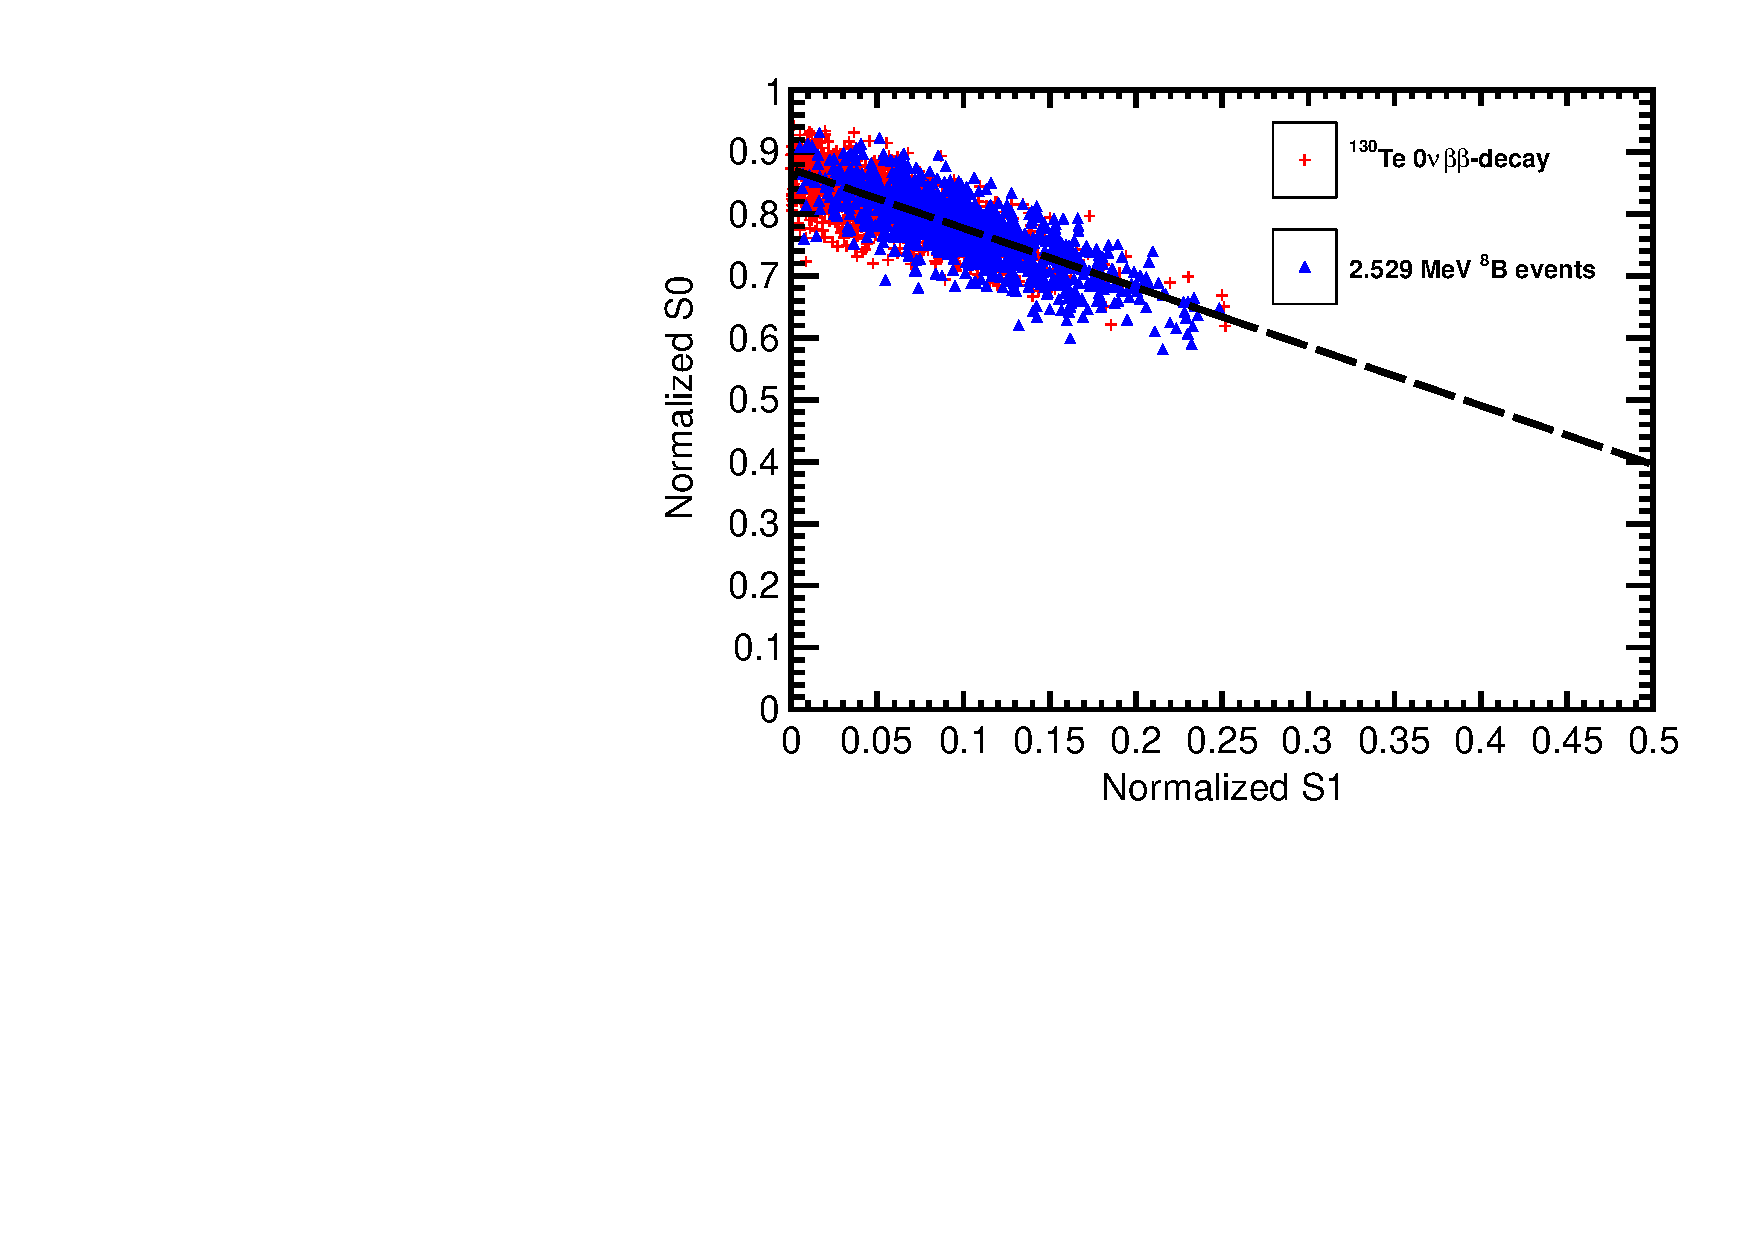
\includegraphics[width=0.49\textwidth]{hS0vsS1_Te130_1el_allLight_VtxSmear0cm_VtxShiftX0cm_momDT1p0ns_rndVtx_3p0mSphere.pdf}
  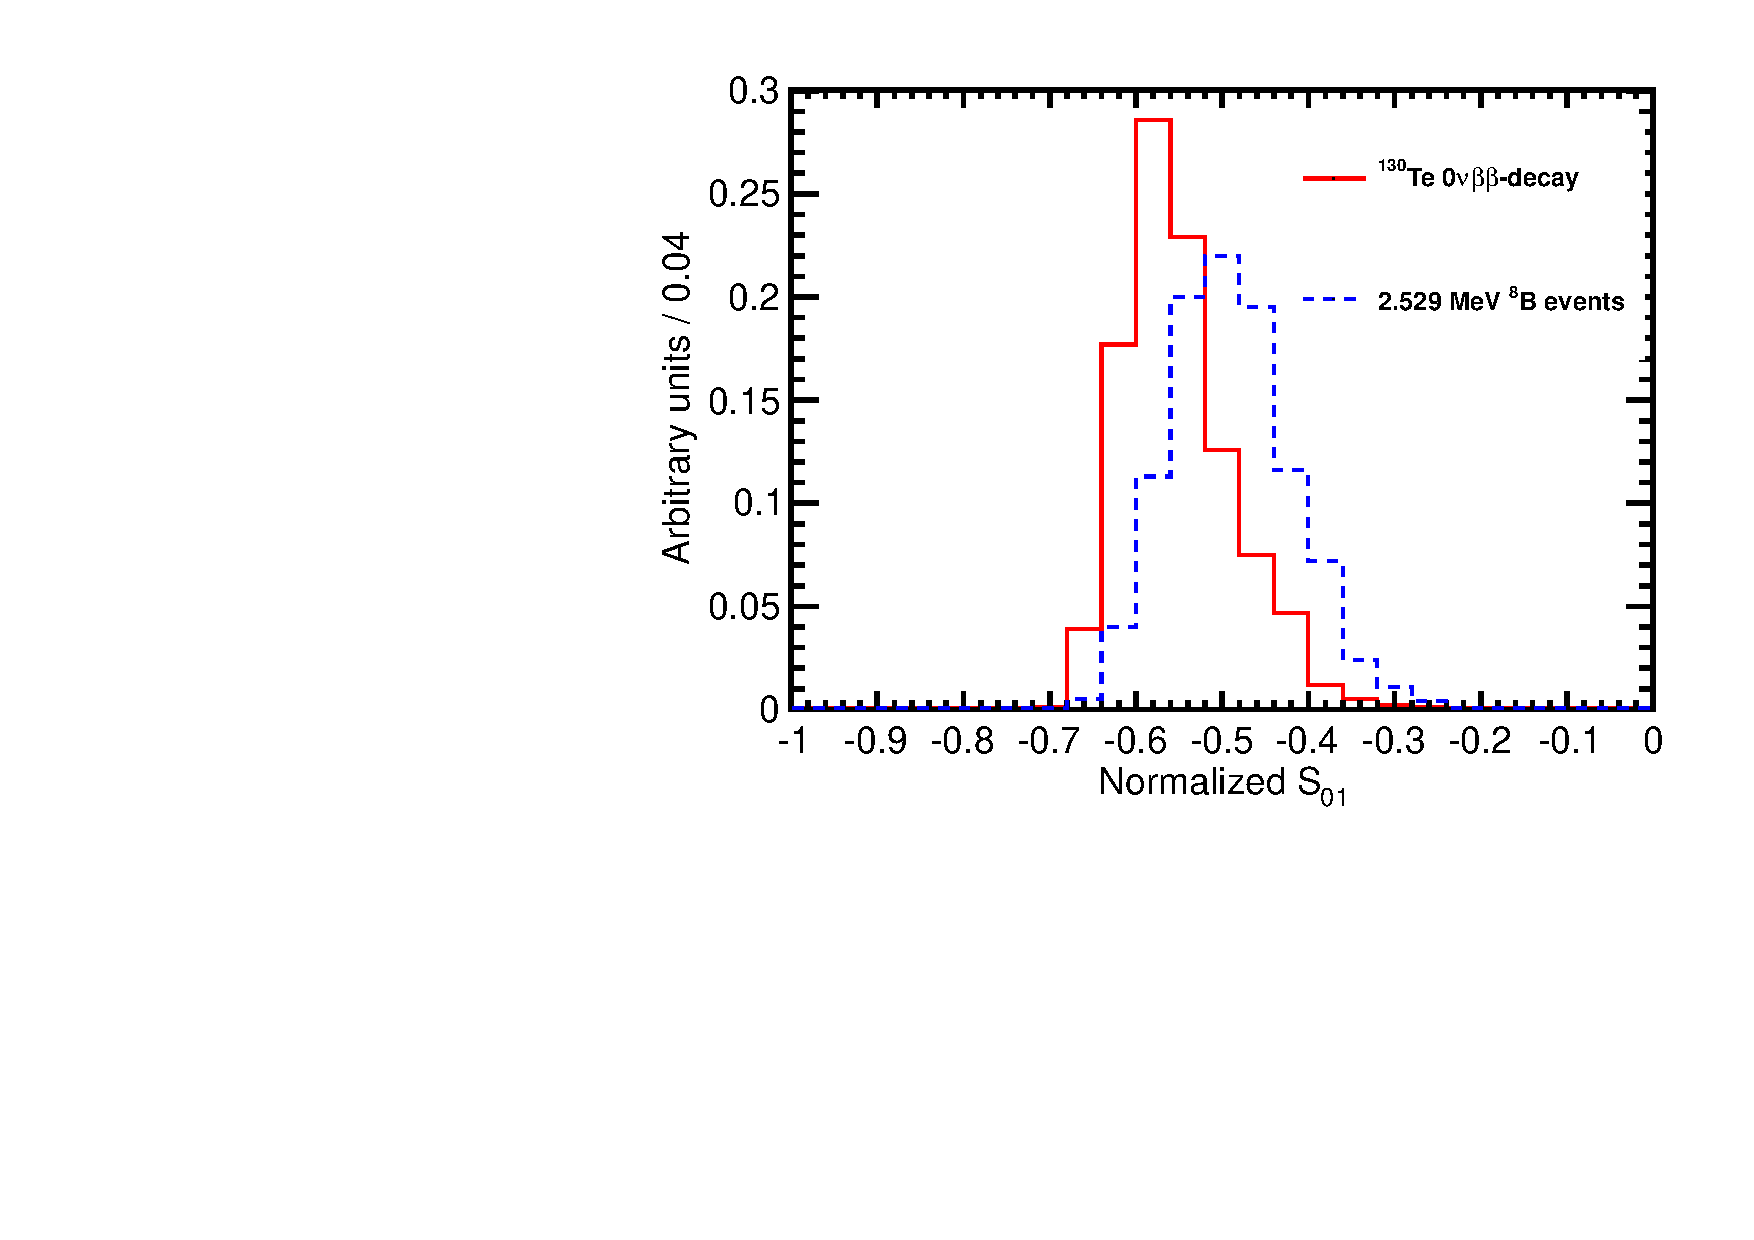
\includegraphics[width=0.49\textwidth]{hS01_allLight_VtxSmear0cm_VtxShiftX0cm_momDT1p0ns_rndVtx_3p0mSphere.pdf}
  \caption{\emph{Left:} Scatter plot of $S_0$ versus $S_1$ for a simulation of 1000 signal (\emph{red crosses}) and background
    (\emph{blue triangles}) events. Event verticies are uniformly distributed within the fiducial volume, $R<3$~m.
    Perfect reconstruction of the vertex position is assumed. Differential cut of 
    $\Delta t=t^{phot}_{measured} - t^{phot}_{predicted}<$1~ns is applied to select early PE sample.
    The default QE and 100\% photo-coverage is used in the simulation.
    Black dashed line corresponds to a linear fit to define 1-D variable $S_{01}$ (see text for details).
    \emph{Right:} Comparison of the $S_{01}$ distribution between signal (\emph{red solid line}) and background (\emph{blue dashed line}).}
  \label{fig:SL_Te_SmearX0cm_momDT1ns_rndVtx_3p0m}
\end{figure*}


\textbf{Text below hasn't been revised yet.}
Imprecise knowledge of the vertex position due to finite resolution is the second factor affecting performance of the spherical 
harmonics analysis. Uncertainty on the vertex position...

The vertex resolution not only reduces Cherenkov/scintillation light separation but it also affects the uniformity 
of the scintillation light distribution in the early PE sample.

Small deviations in vertex reconstruction cause a large effect
on the $S_0$ and $S_1$ distributions for the single electron event topology.
For the vertices shifted along the direction of the electron track the relative time cut $\Delta t$
reduces the uniformity of the scintillation light distribution. The
$\Delta t$ cut selects more forward emitted photons in the case when
the reconstructed vertex is shifted to the direction opposite to the
electron momentum. This enhances the forward region populated by Cherenkov
photons and causes a more asymmetric photon distribution that moves $S_1$ to higher values.  The opposite occurs for the case where the reconstructed vertex is shifted in the direction along the electron
momentum. Here, the time cut selects more backward emitted photons and counter balances the forward region populated by Cherenkov
photons leading to a more symmetric photon distribution and smaller values of $S_1$.

Figure~\ref{fig:SL_Te_SmearX3cm_momDT1ns_rndVtx_3p0m} shows the performance of the spherical harmonics analysis for events after taking into account a 3~cm vertex reconstruction resolution, applied uniformly within the fiducial volume. Since the goal of this paper is to introduce spherical harmonic analysis we do not perform a full vertex reconstruction and only apply smearing to the simulated vertex position using a Gaussian distribution with sigma of 3~cm on $x$, $y$, and $z$ coordinates. 

\begin{figure*}[h]
  \centering
  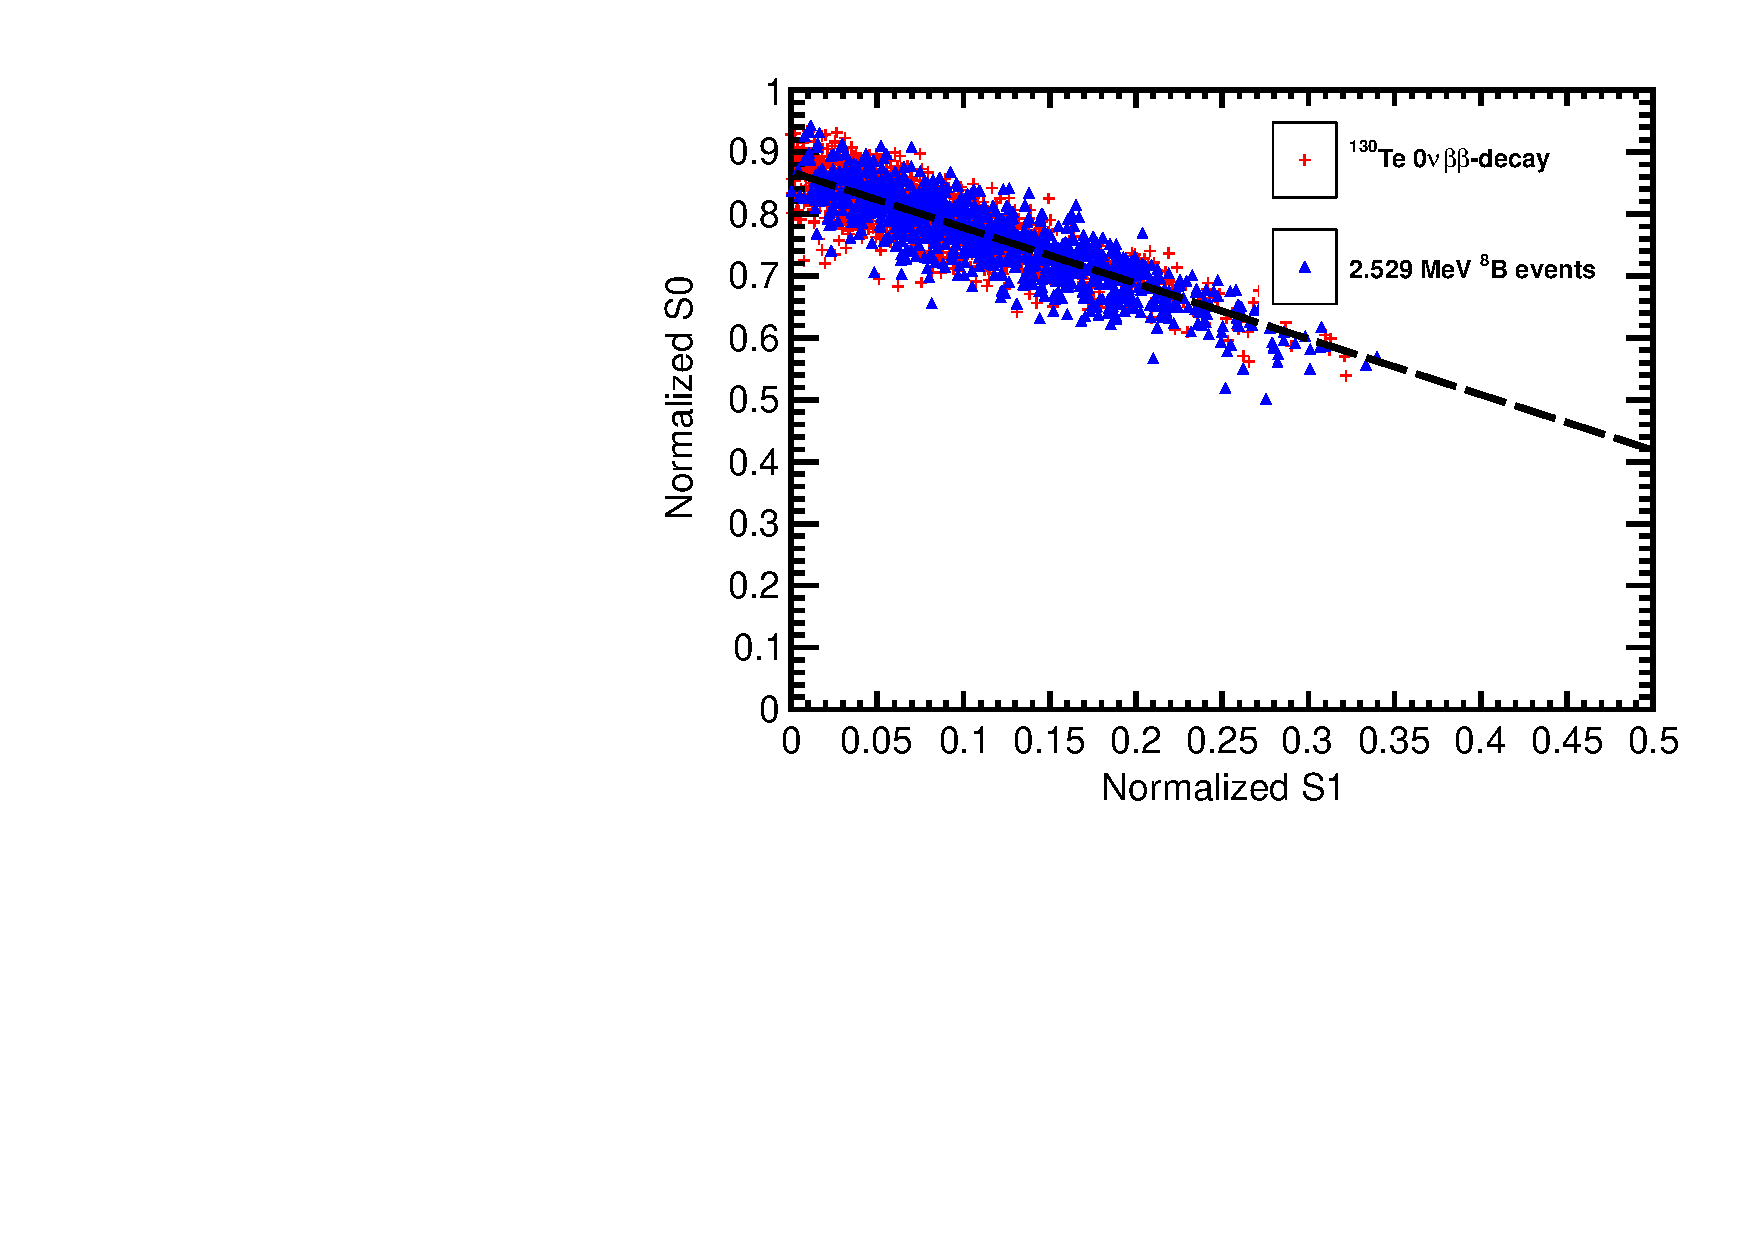
\includegraphics[width=0.49\textwidth]{hS0vsS1_Te130_1el_allLight_VtxSmear3cm_VtxShiftX0cm_momDT1p0ns_rndVtx_3p0mSphere.pdf}
  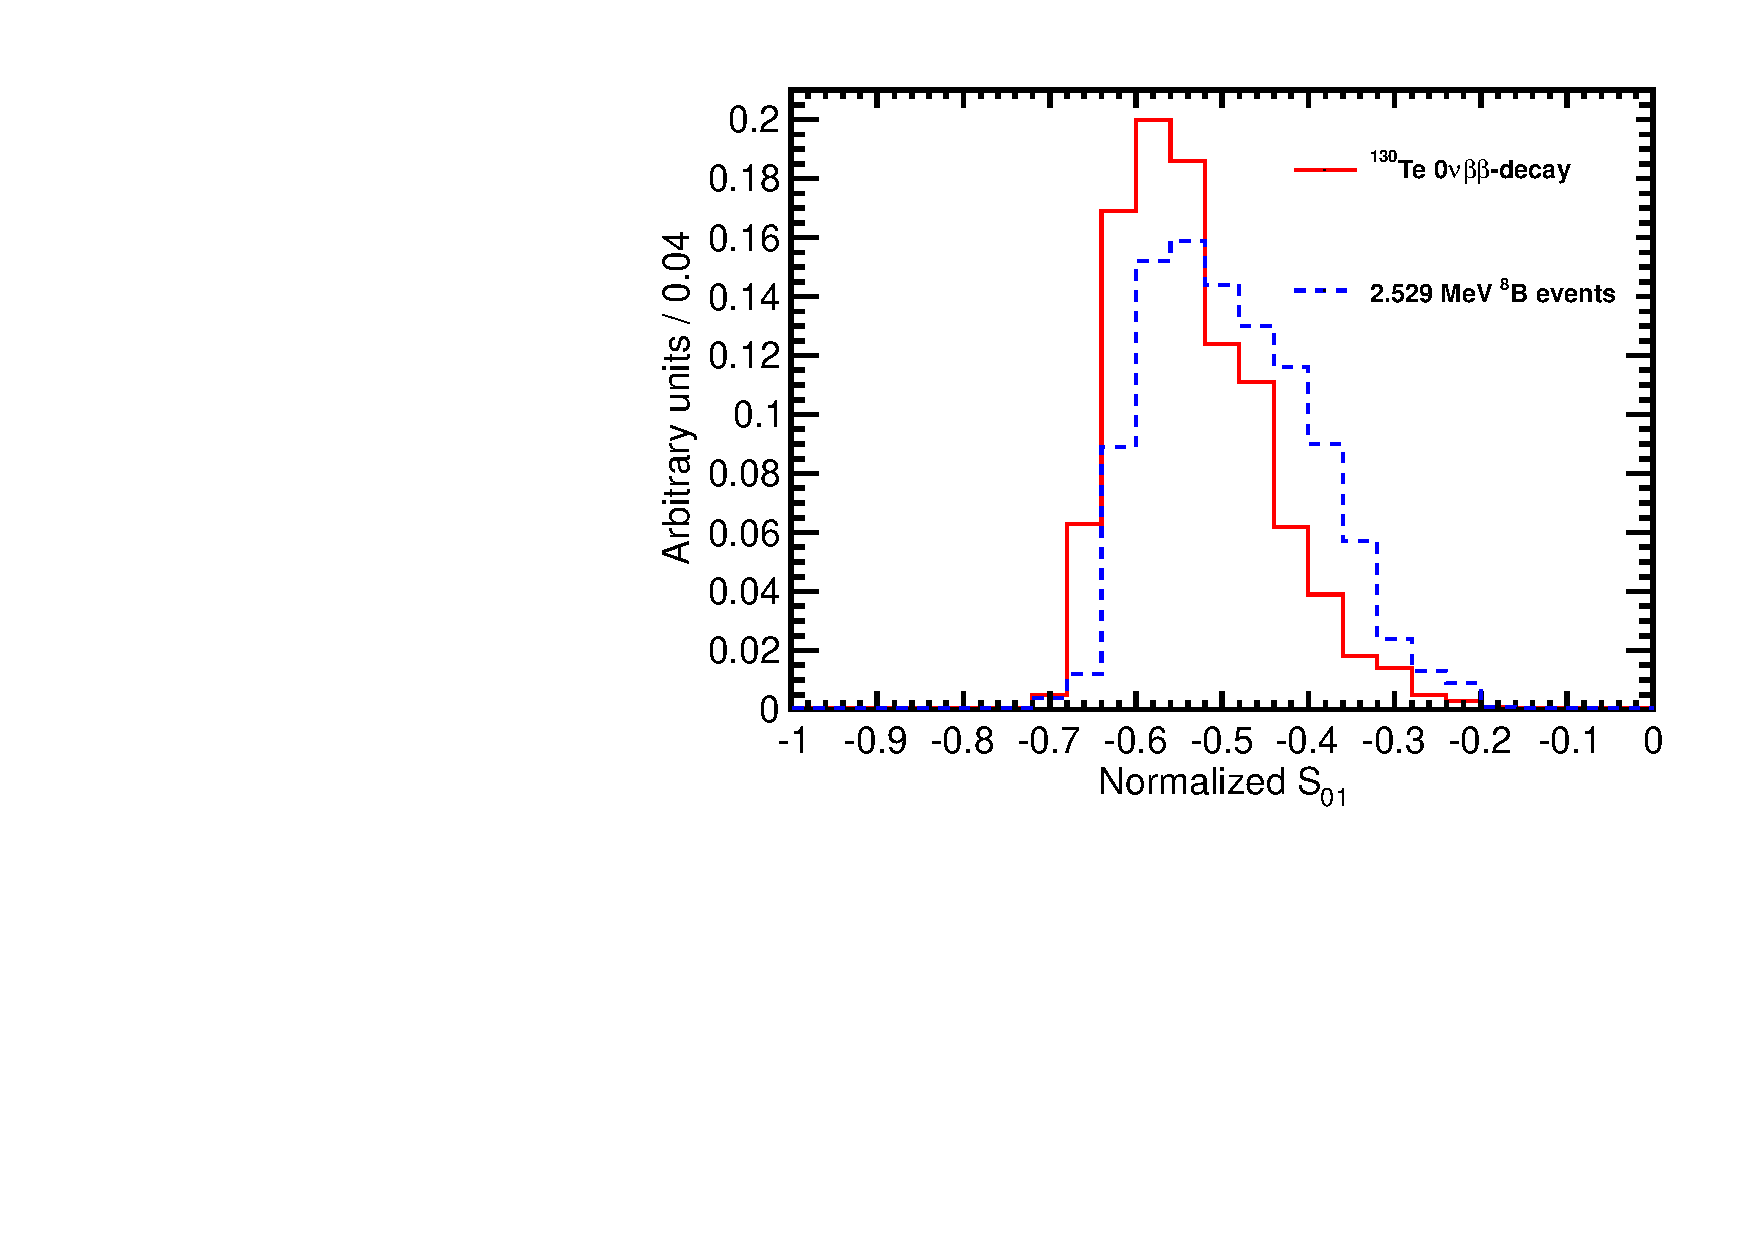
\includegraphics[width=0.49\textwidth]{hS01_allLight_VtxSmear3cm_VtxShiftX0cm_momDT1p0ns_rndVtx_3p0mSphere.pdf}
  \caption{Spherical harmonics comparison between $^{130}$Te 0{\nbb}
    decay signal ($Q=2.529$~MeV) (\emph{red}) and $^{8}$B solar
    neutrinos background (\emph{blue}) for 1000 simulated
    events.Verticies are uniformly distributed within the fiducial
    volume, R$<$3~m. $^8$Be events are implemented as 2.529~MeV
    electrons with the initial momentum direction uniformly
    distributed within 4$\pi$ solid angle. Vetrex is smeared with 3~cm
    resolution. \emph{Left:} $S_0$ versus $S_1$ scatter plot. Black
    dotted line is a linear fit of these 2D histograms. Variable
    $S_{01}$ is defined as a projection of 2D distribution onto this
    linear fit. \emph{Right:} $S_{01}$}
\label{fig:SL_Te_SmearX3cm_momDT1ns_rndVtx_3p0m}
\end{figure*}


{\bf Solution to this problem would be a better selection criteria of
  early light. It has to preserve high admixture of the Cherenkov
  photons, but needs to select scintillation photons in a more uniform
  manner. Working on it, but may not be simple so I don't want to
  include it in this paper.}

Good vertex resolution is essential for spherical harmonics analysis. As one can see in Fig.~\ref{fig:SL_Te_SmearX3cm_momDT1ns_rndVtx_3p0m}, even a 3~cm vertex resolution reduces the discrimination power of the spherical harmonics analysis.

Such strong dependence on the vertex resolution can be
addressed by choosing a different liquid scintillator mixture with a
more delayed emission of the scintillation light with respect to the Cherenkov light. With a larger delay in the scintillation light, a high fraction of Cherenkov light in the early PE sample selected with relative time cut $\Delta t$ can be maintained for a given vertex resolution. In addition, if the fraction of scintillation light is small compared to Cherenkov light, the distortions in the uniformity of the scintillation light distribution due to mis-reconstructed vertex do not significantly affect the $S_0$ and $S_1$ variables.

Figure~\ref{fig:SL_Te_momDT1ns_sci0p5ns_rndVtx_3p0m} shows
spherical harmonics analysis for the simulation where the
scintillation component is delayed by an additional 0.5ns compared to our default simulation. Events are simulated uniformly within the fiducial volume of the detector. Vertex resolution of 3~cm is assumed. Noticeable separation between \nbb and \B~events is achieved.

The discrimination power of the spherical harmonics analysis improves with vertex resolution and more delay in the emission of the scintillation light. Moreover the dependence on vertex reconstruction reduces with delay in the scintillation light. 

\begin{figure*}[h]
  \centering
  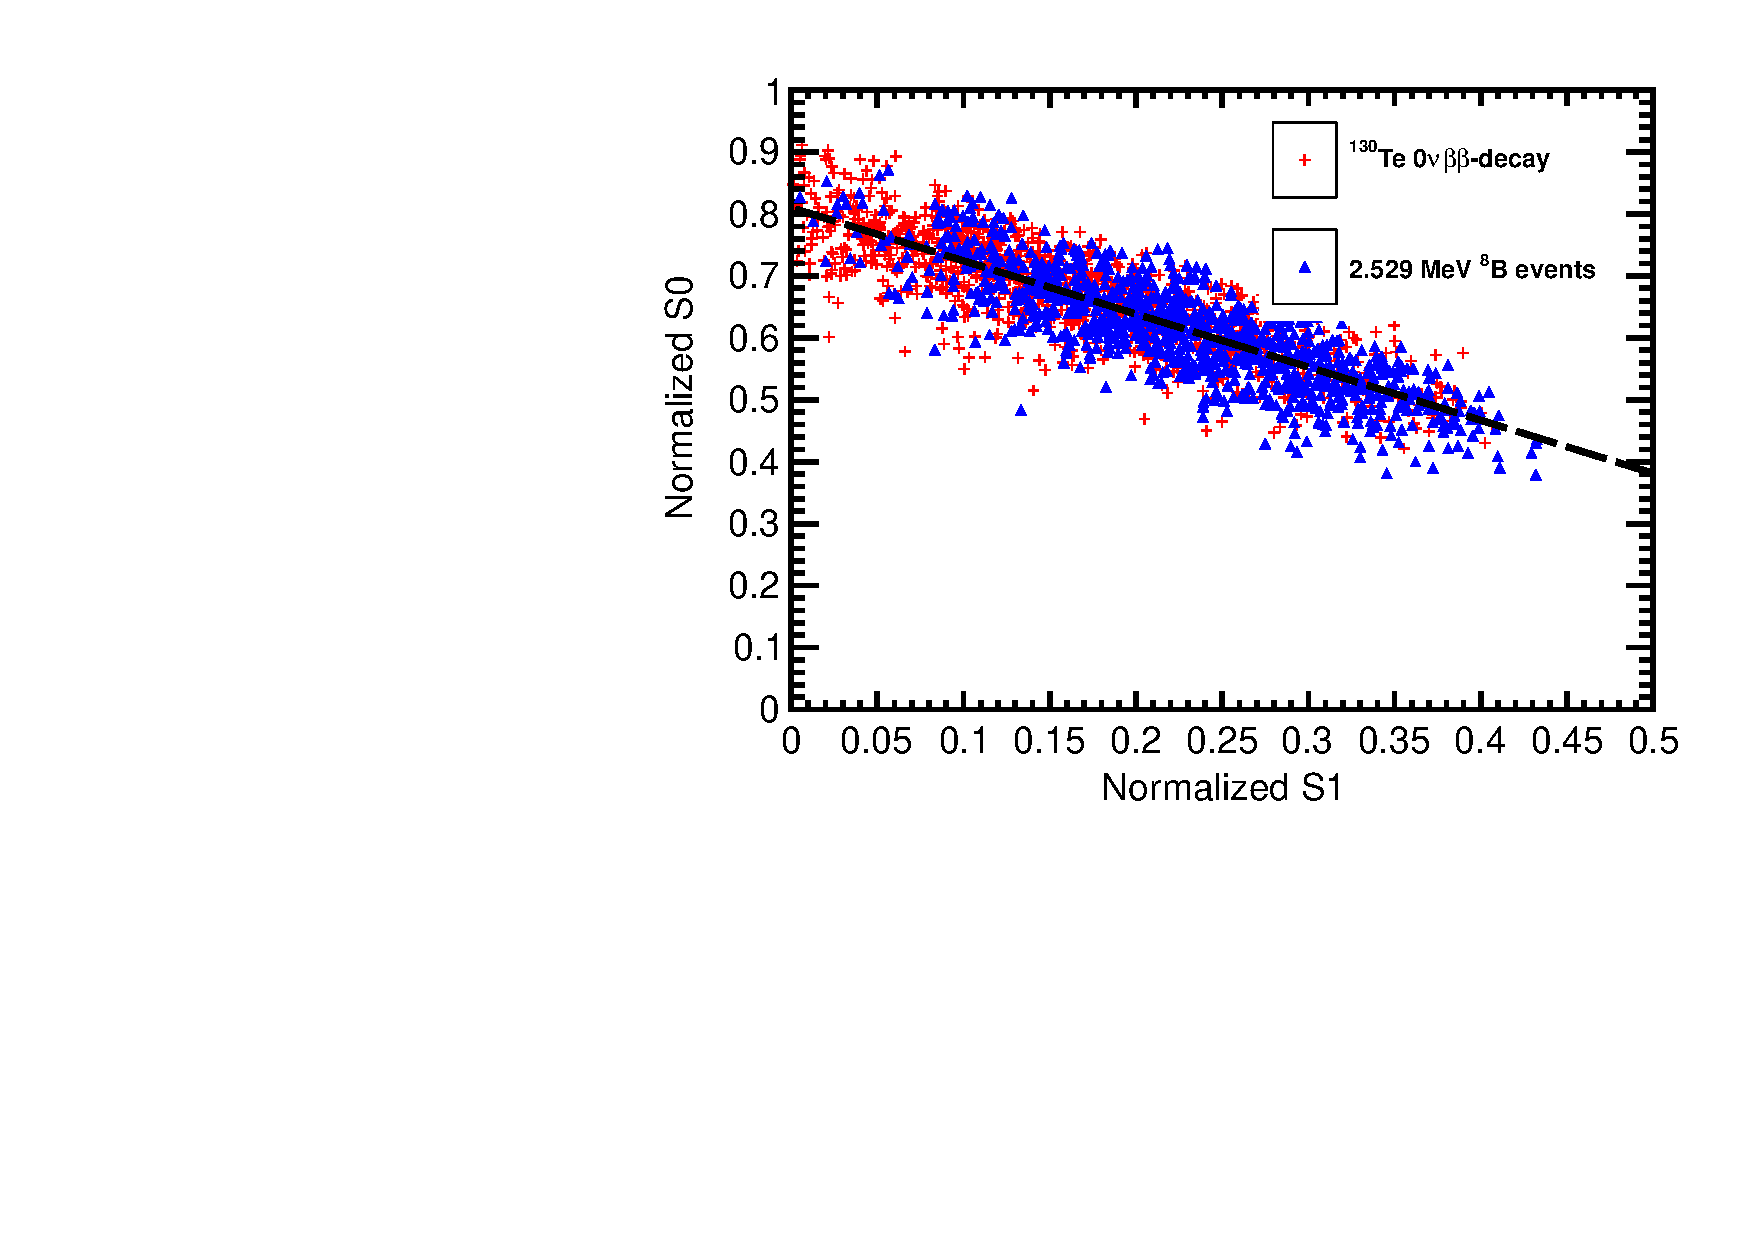
\includegraphics[width=0.49\textwidth]{hS0vsS1_Te130_1el_allLight_VtxSmear3cm_VtxShiftX0cm_momDT1p0ns_sci0p5ns_rndVtx_3p0mSphere.pdf}
  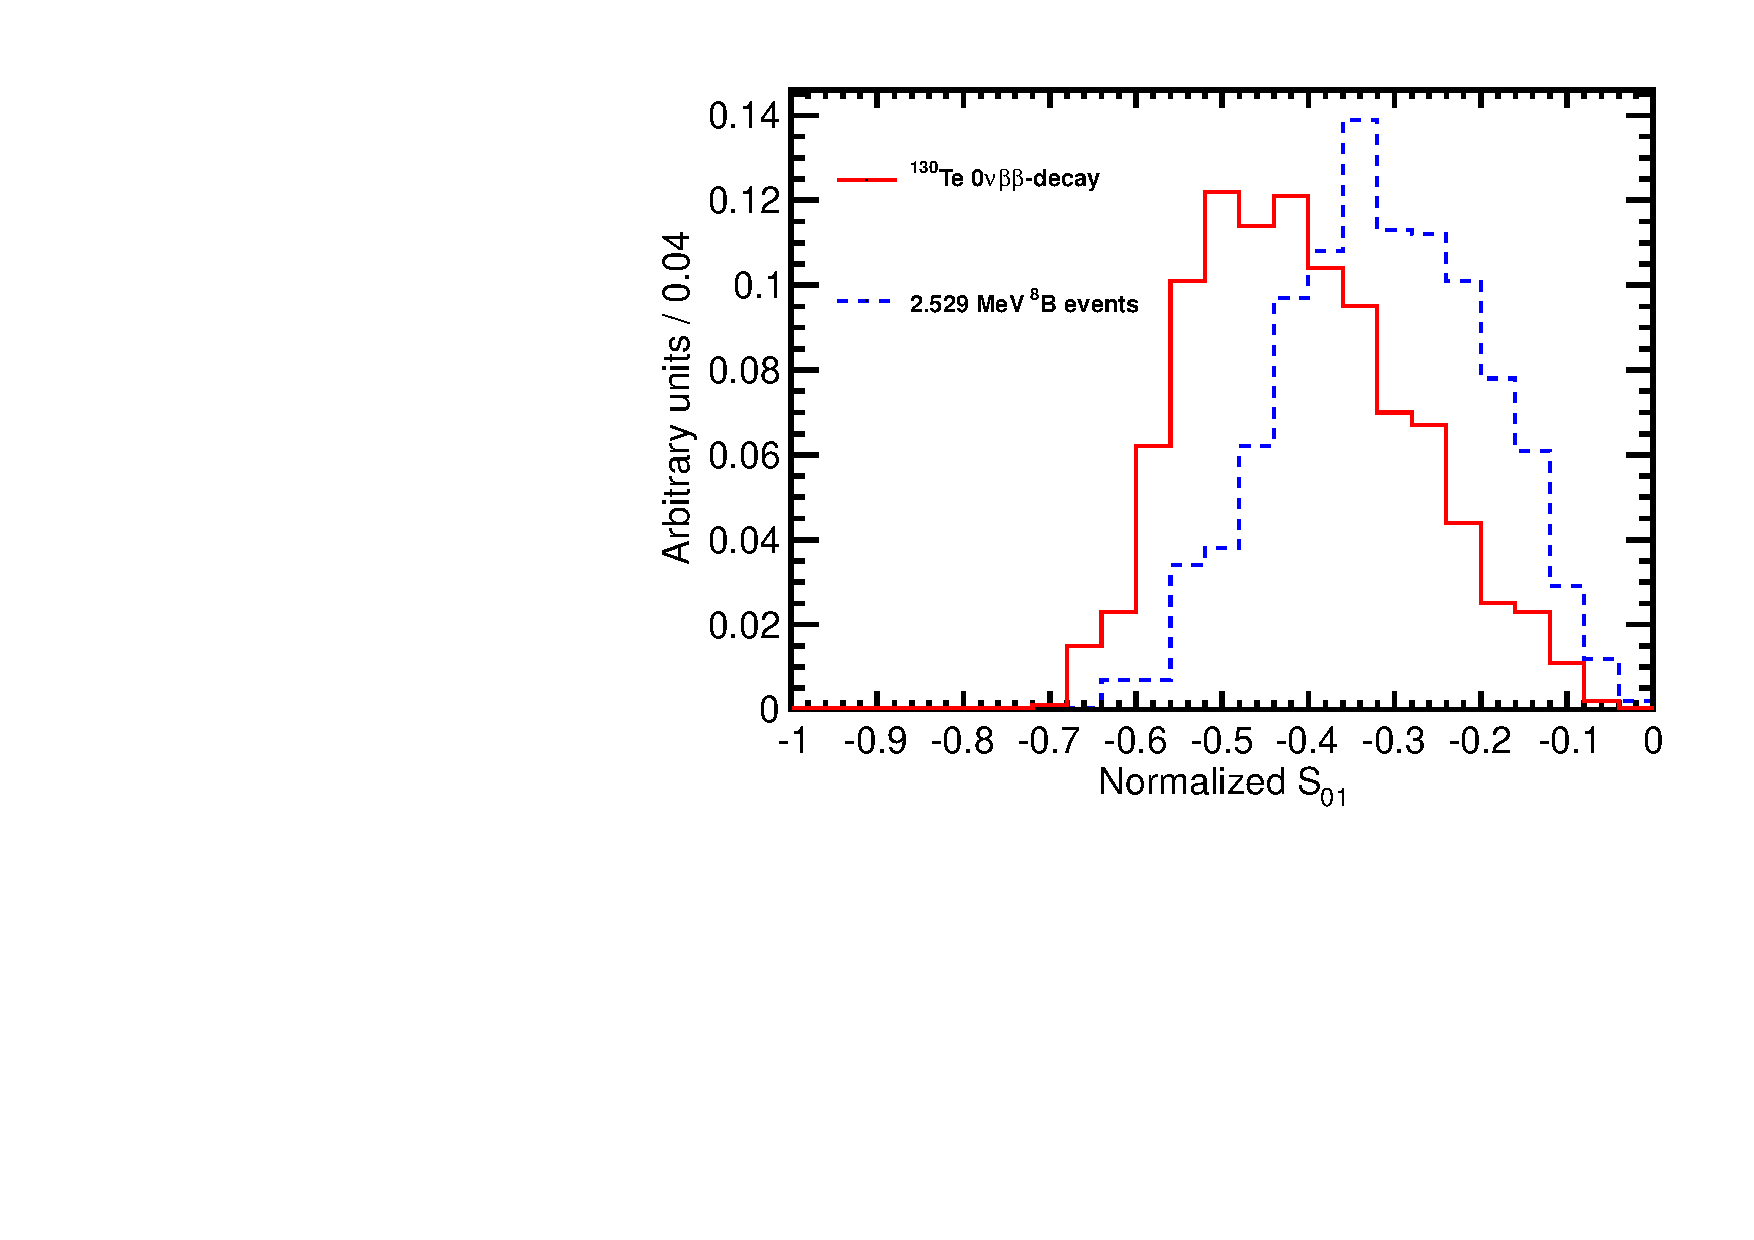
\includegraphics[width=0.49\textwidth]{hS01_allLight_VtxSmear3cm_VtxShiftX0cm_momDT1p0ns_sci0p5ns_rndVtx_3p0mSphere.pdf}
  \caption{Spherical harmonics comparison between $^{130}$Te 0{\nbb}
    decay signal ($Q=2.529$~MeV) (\emph{red}) and $^{8}$B solar
    neutrinos background (\emph{blue}) for 1000 simulated
    events. Verticies are uniformly distributed within the fiducial
    volume, $R<3$~m. $^8$Be events are implemented as 2.529~MeV
    electrons with the initial momentum direction uniformly
    distributed within 4$\pi$ solid angle. Vetrex is smeared with 3~cm
    resolution. {\bf Scintillation light is delayed by additional
      0.5~ns.} \emph{Left:} $S_0$ versus $S_1$ scatter plot. Black dotted
    line is a linear fit of these 2D histograms. Variable $S_{01}$ is
    defined as a projection of 2D distribution onto this linear
    fit. \emph{Right:} $S_{01}$}
\label{fig:SL_Te_SmearX3cm_momDT1ns_sci0p5ns_rndVtx_3p0m}
\end{figure*}

Next generation LS detectors may be able to recover theses losses due to chromatic dispersion by choosing liquid scintillators with a more narrow emission spectrum (e.g. see Ref~\cite{LS_narrow_emission}). Etc...

